\documentclass[aspectratio=169,10pt]{beamer}
\usetheme{Madrid}
\usecolortheme{seahorse}
\setbeamertemplate{footline}[frame number]

\usepackage[utf8]{inputenc}
\usepackage{amsmath,amssymb,amsthm}
\usepackage{graphicx}
\usepackage{listings}
\usepackage{xcolor}
\usepackage{tikz}

\graphicspath{{figures/}}

\lstset{
  basicstyle=\ttfamily\scriptsize,
  numbers=left,
  frame=single,
  backgroundcolor=\color{gray!7},
  keywordstyle=\color{blue}\bfseries,
  commentstyle=\color{green!50!black}\itshape,
  stringstyle=\color{red!60!black},
  breaklines=true,
  showstringspaces=false,
  language=Python
}

\newcommand{\B}{\mathbb{B}}
\newcommand{\N}{\mathbb{N}}
\newcommand{\R}{\mathbb{R}}
\newcommand{\Z}{\mathbb{Z}}
\newcommand{\Q}{\mathbb{Q}}
\newcommand{\E}{\mathbb{E}}
\newcommand{\PP}{\mathbb{P}}

\title{Background: Miscellaneous, History and References}
\subtitle{Sections 2.8 -- 2.9}
\author{Chapter 2 --- Background}
\institute{An Introduction to Universal Artificial Intelligence \\ \small Hutter, Quarel, Catt (2024)}
\date{}

\begin{document}

% ============================================================
\begin{frame}
  \titlepage
\end{frame}

% ============================================================
\begin{frame}{Outline}
  \tableofcontents
\end{frame}

\section{2.8 Miscellaneous: Overview}

% ============================================================
\begin{frame}{What This Section Is For}
  Section 2.8 collects material that quietly underlies the rest of the book,
  but which is more of a technical toolbox than essential reading on a first
  pass. It is organized into three parts.

  \begin{block}{2.8.1 Distances and their relation}
    Several different notions of ``distance'' between two probability
    distributions (absolute, squared, KL, Hellinger) are introduced, and we
    prove that the Kullback--Leibler (KL) divergence upper-bounds all the
    others. This lets us prove one bound and get several bounds for free.
  \end{block}

  \begin{block}{2.8.2 Dealing with semimeasures}
    A \emph{semimeasure} is a relaxation of a probability measure that allows
    total probability to be less than 1 (some mass can be ``missing''). This
    subsection lists workarounds for the extra technical headaches
    semimeasures cause.
  \end{block}

  \begin{block}{2.8.3 Probability zero}
    How to sensibly define conditional probabilities and expectations when we
    condition on an event that has probability exactly zero.
  \end{block}
\end{frame}

\section{2.8.1 Distances and Their Relation}

% ============================================================
\begin{frame}{Why We Need Multiple Notions of Distance}
  Throughout the book (and especially in Chapter 3) we need to measure how
  ``far apart'' two probability distributions $P$ and $Q$ are. Several
  different distances are useful, each with its own pros and cons:

  \begin{itemize}
    \item \textbf{Absolute distance} (twice the total variation distance):
      a proper metric, very natural for probability measures.
    \item \textbf{Squared distance} (square of the Euclidean distance): the
      most common choice, but often the least suitable one (see the
      exercises).
    \item \textbf{KL divergence} (Section 2.5.3): not a metric (it is not
      symmetric and can be infinite), but it is the
      information-theoretically most useful quantity for proving bounds.
    \item \textbf{(Squared) Hellinger distance}: another proper metric,
      useful in some later chapters.
  \end{itemize}

  \textbf{Key idea of this subsection.} KL divergence is an upper bound to
  all the other distances, while at the same time being a lower bound for
  many loss functions used later in the book. This makes it an extremely
  useful hub through which to route proofs. We restrict attention to finite
  sample spaces $\Omega$, where probabilities are $d$-dimensional vectors in
  the probability simplex.
\end{frame}

% ============================================================
\begin{frame}{Lemma 2.8.1: Pinsker's Binary Inequality}
  \begin{block}{Lemma 2.8.1 (Pinsker's binary inequality)}
    For $0 \le p, q \le 1$,
    \[
      2(p-q)^2 \;\le\; p\ln\frac{p}{q} + (1-p)\ln\frac{1-p}{1-q}.
    \]
  \end{block}

  \textbf{Plain English.} Think of $p = P(1)$ and $q = Q(1)$ as the
  probabilities that two coins (biased distributions $P$ and $Q$ over
  $\{0,1\}$) land on ``1''. The right-hand side is exactly the KL divergence
  between $P$ and $Q$. The lemma says: twice the squared gap between the two
  coin biases is never bigger than their KL divergence. In other words, KL
  divergence controls (upper-bounds) the simpler squared distance.

  \vspace{2mm}
  There are many known proofs of this inequality, none of them particularly
  illuminating; we present the shortest one.
\end{frame}

% ============================================================
\begin{frame}[allowframebreaks]{Proof of Pinsker's Binary Inequality}
  \textbf{Proof.} Define $f(x) = p\ln x + (1-p)\ln(1-x)$. Then
  \[
    p\ln\frac{p}{q} + (1-p)\ln\frac{1-p}{1-q} \;=\; f(p) - f(q).
  \]
  \textbf{Plain English.} $f$ is just a convenient helper function built from
  $p$; subtracting $f$ at two points $p$ and $q$ reproduces exactly the KL
  term we want to bound.

  Also note that for $0\le x\le 1$ we have $x(1-x) \le 1/4$ (the maximum of
  $x(1-x)$ on $[0,1]$ is $1/4$, attained at $x=1/2$). Then
  \[
    f(p) - f(q) \;=\; \int_q^p f'(x)\,dx \;=\; \int_q^p \frac{p-x}{x(1-x)}\,dx
    \;\ge\; 4\int_q^p (p-x)\,dx \;=\; 2(p-q)^2. \qquad\blacksquare
  \]
  \textbf{Plain English.} We rewrite the difference $f(p)-f(q)$ as an
  integral of the derivative $f'$, then use $x(1-x)\le 1/4$ (so
  $1/(x(1-x)) \ge 4$) to lower-bound the integrand, and finally evaluate the
  resulting simple integral to get exactly $2(p-q)^2$.

  \begin{center}
    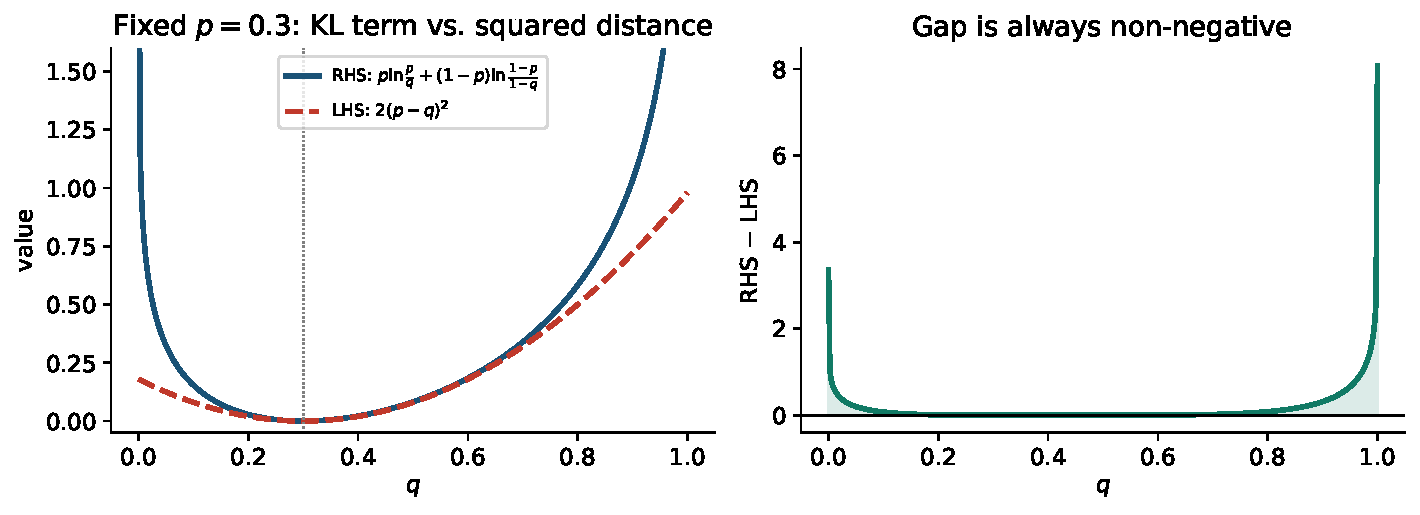
\includegraphics[width=0.82\textwidth]{pinsker}
  \end{center}
  \textit{Left: both sides of the inequality as functions of $q$, for fixed
  $p=0.3$. Right: their gap, always non-negative.}
\end{frame}

% ============================================================
\begin{frame}{Lemma 2.8.2: Convex Even Functions Are Monotonic on $\mathbb{R}^+$}
  \begin{block}{Lemma 2.8.2 (Convex even functions are monotonic on $\mathbb{R}^+$)}
    Let $f:\mathbb{R}\to\mathbb{R}$ be an \emph{even} convex function (i.e.\
    $f(x) = f(-x)$ for all $x$). Then $f$ is monotonically increasing over
    the positive reals.
  \end{block}

  \textbf{Plain English.} ``Convex'' means the graph of $f$ curves upward
  (a chord between two points on the graph lies above the graph); ``even''
  means the graph is symmetric about the vertical axis, like $f(x)=x^2$ or
  $f(x)=|x|$. The lemma says any such function, restricted to positive
  inputs, can only go up (or stay flat) as its input increases --- it is a
  purely geometric fact used repeatedly in the next few results.
\end{frame}

% ============================================================
\begin{frame}[allowframebreaks]{Proof of Lemma 2.8.2}
  \textbf{Proof.} Take the definition of convexity,
  $f(\alpha x + (1-\alpha)y) \le \alpha f(x) + (1-\alpha)f(y)$ for
  $0\le\alpha\le 1$, and insert $x = a+b$, $y=0$:
  \begin{equation}
    f(\alpha(a+b)) \;\le\; \alpha f(a+b) + (1-\alpha) f(0). \tag{2.8.3}
  \end{equation}
  \textbf{Plain English.} $\alpha$ (alpha) is a mixing weight between $0$
  and $1$; this is just the convexity inequality applied to the two specific
  points $a+b$ and $0$.

  Now, assuming $a,b\ge 0$, insert $\alpha = \frac{a}{a+b} \ge 0$ or
  $\alpha = \frac{b}{a+b} \ge 0$ to get two inequalities:
  \[
    f(a) \;\le\; \frac{a}{a+b}f(a+b) + \frac{b}{a+b}f(0), \qquad
    f(b) \;\le\; \frac{b}{a+b}f(a+b) + \frac{a}{a+b}f(0).
  \]
  Adding the two:
  \begin{equation}
    f(a) + f(b) \;\le\; f(a+b) + f(0). \tag{2.8.4}
  \end{equation}

  \framebreak

  Also, in (2.8.3) choose $\alpha = 1/2$, $x=-b$, $y=b$, to obtain
  \[
    f(0) \;\le\; \tfrac12 f(b) + \tfrac12 f(-b) \;=\; f(b)
  \]
  since $f$ is even (so $f(-b)=f(b)$).

  \textbf{Plain English.} Plugging in a mix of $-b$ and $b$ (which averages
  to $0$) into the convexity inequality tells us $f(0)$ can never exceed
  $f(b)$.

  Substituting $f(0)\le f(b)$ into (2.8.4), $f(a)+f(b) \le f(a+b)+f(0) \le
  f(a+b)+f(b)$, and cancelling $f(b)$ from both sides gives
  \[
    f(a) \;\le\; f(a+b),
  \]
  which proves $f$ is monotonically increasing for positive arguments.
  $\blacksquare$
\end{frame}

% ============================================================
\begin{frame}{Lemma 2.8.5: Convex Even Functions Are Subadditive}
  \begin{block}{Lemma 2.8.5 (Convex even functions are subadditive)}
    Let $f$ be an even convex function such that $f(0)\le 0$. Then
    \[
      f(a) + f(b) \;\le\; f(a+b) \qquad \text{for all } a,b \ge 0.
    \]
  \end{block}

  \textbf{Plain English.} ``Subadditive'' means applying $f$ to a sum is at
  least as large as summing $f$ applied separately: the function doesn't
  ``lose value'' when you combine its arguments. This follows immediately
  from (2.8.4) once we additionally know $f(0)\le 0$: then
  $f(a)+f(b) \le f(a+b)+f(0) \le f(a+b)$.
  $\blacksquare$

  \vspace{3mm}
  This innocuous-looking lemma is the key technical ingredient for the main
  result of this subsection: a single inequality that, depending on which
  convex even function $f$ we plug in, yields a bound for several different
  distances at once.
\end{frame}

% ============================================================
\begin{frame}{Theorem 2.8.6: General Entropy Inequality}
  \begin{block}{Theorem 2.8.6 (General entropy inequality) [Hut05b, Sec.\ 3.9.2]}
    Let $(y_1,\ldots,y_d)$ and $(z_1,\ldots,z_d)$ be elements of a
    $d$-dimensional (semi)probability simplex, i.e.\ $y_i\ge 0$ with
    $\sum_i y_i = 1$ (and $z_i \ge 0$ with $\sum_i z_i \le 1$). Then for any
    function $f:\mathbb{R}\to\mathbb{R}$ that is convex, even, and satisfies
    $f(0)\le 0$, we have
    \[
      \frac12 \sum_{i=1}^d f(y_i - z_i) \;\le\; f\!\left(\sqrt{\frac12
      \sum_{i=1}^d y_i \ln\frac{y_i}{z_i}}\right).
    \]
  \end{block}

  \textbf{Plain English.} $y_i$ and $z_i$ are the probabilities that two
  distributions $Y$ and $Z$ assign to outcome $i$, out of $d$ possible
  outcomes. The right-hand inner expression $\sum_i y_i \ln(y_i/z_i)$ is the
  KL divergence between $Y$ and $Z$. The theorem says: for \emph{any} convex,
  even ``distance-shape'' function $f$ (with $f(0)\le 0$), the total
  per-outcome discrepancy $f(y_i-z_i)$, summed and halved, is bounded by $f$
  applied to the square root of half the KL divergence. Plugging in
  different choices of $f$ below gives several concrete, familiar distance
  bounds ``for free''.
\end{frame}

% ============================================================
\begin{frame}[allowframebreaks]{Proof of Theorem 2.8.6}
  \textbf{Proof.} Let $I=\{1,\ldots,d\}$. Partition $I = P \dot\cup Q$ into
  two disjoint sets. For $S \in \{P,Q\}$, define $y^S := \sum_{i\in S} y_i$
  and $z^S := \sum_{i\in S} z_i$, and normalize $p_i^S := y_i/y^S$,
  $q_i^S := z_i/z^S$ for $i \in S$; these are valid probability
  distributions on $S$.

  By Gibbs' inequality (Theorem 2.5.15, which says KL divergence is always
  $\ge 0$),
  \[
    0 \;\le\; \sum_{i\in S} p_i^S \ln\frac{p_i^S}{q_i^S}
    \;=\; \frac{1}{y^S}\sum_{i\in S} y_i \ln\frac{y_i}{z_i}
    \;-\; \frac{1}{y^S}\sum_{i\in S} y_i \ln\frac{y^S}{z^S},
  \]
  hence $\sum_{i\in S} y_i \ln\frac{y_i}{z_i} \ge y^S \ln\frac{y^S}{z^S}$.

  \framebreak

  Noting $y^Q = 1-y^P$ and $z^Q \le 1-z^P$, and summing the $P$ and $Q$
  contributions,
  \[
    \sum_{i=1}^d y_i \ln\frac{y_i}{z_i} \;\ge\;
    y^P\ln\frac{y^P}{z^P} + y^Q\ln\frac{y^Q}{z^Q}
    \;\ge\; y^S\ln\frac{y^S}{z^S} + (1-y^S)\ln\frac{1-y^S}{1-z^S}
    \;\ge\; 2(y^S-z^S)^2,
  \]
  where the last step is exactly Pinsker's binary inequality (Lemma 2.8.1)
  applied with $p=y^S,q=z^S$. Therefore
  \begin{equation}
    (y^S - z^S)^2 \;\le\; \frac12 \sum_{i=1}^d y_i \ln\frac{y_i}{z_i}. \tag{2.8.7}
  \end{equation}

  \framebreak

  Now choose $P = \{i\in I: y_i > z_i\}$ and $Q = \{i \in I : y_i \le z_i\}$,
  and bound $\sum_{i\in S} f(y_i-z_i)$:
  \[
    \sum_{i\in S} f(y_i-z_i)
    \;\overset{(a)}{=}\; \sum_{i\in S} f(|y_i-z_i|)
    \;\overset{(b)}{\le}\; f\Big(\sum_{i\in S}|y_i-z_i|\Big)
    \;\overset{(c)}{=}\; f\Big(\Big|\sum_{i\in S}y_i-z_i\Big|\Big)
    \;\overset{(d)}{=}\; f(|y^S-z^S|)
  \]
  \[
    \;=\; f\big(\sqrt{(y^S-z^S)^2}\big) \;\overset{(e)}{\le}\;
    f\!\left(\sqrt{\tfrac12\sum_{i=1}^d y_i\ln\frac{y_i}{z_i}}\right).
  \]
  \textbf{Plain English of steps.} (a) $f$ is even, so $f(x)=f(|x|)$.
  (b) Lemma 2.8.5 (subadditivity of $f$). (c) By construction of $S$, all
  the terms $y_i-z_i$ inside $S$ share the same sign, so we may sum first,
  then take the absolute value. (d) Distribute the sum. (e) Apply (2.8.7)
  together with monotonicity of $\sqrt{\cdot}$ and of $f$ (Lemma 2.8.2).

  \framebreak

  Finally, we conclude by combining the bound for $P$ and $Q$:
  \[
    \frac12 \sum_{i=1}^d f(y_i-z_i) \;=\; \frac12\sum_{i\in P} f(y_i-z_i) +
    \frac12\sum_{i\in Q} f(y_i-z_i)
    \;\le\; f\!\left(\sqrt{\frac12\sum_{i=1}^d y_i\ln\frac{y_i}{z_i}}\right).
    \qquad \blacksquare
  \]
\end{frame}

% ============================================================
\begin{frame}{Corollary 2.8.8: Specific Entropy Inequalities}
  \begin{block}{Corollary 2.8.8 (Specific entropy inequalities)}
    Continuing from Theorem 2.8.6:
    \begin{align*}
      \text{(S) Square:}      &\quad \sum_{i=1}^d (y_i-z_i)^2 \;\le\; \sum_{i=1}^d y_i\ln\frac{y_i}{z_i} \\
      \text{(A) Absolute:}    &\quad \sum_{i=1}^d |y_i-z_i| \;\le\; \sqrt{2\sum_{i=1}^d y_i\ln\frac{y_i}{z_i}} \\
      \text{(H) Hellinger}^2: &\quad \sum_{i=1}^d (\sqrt{y_i}-\sqrt{z_i})^2 \;\le\; \sum_{i=1}^d y_i\ln\frac{y_i}{z_i}
    \end{align*}
  \end{block}

  \textbf{Plain English.} Each row is one concrete, well-known distance
  between the distributions $Y$ and $Z$, all bounded above by the very same
  KL divergence $\sum_i y_i \ln(y_i/z_i)$. Row (S) is obtained from
  Theorem 2.8.6 by choosing $f(x)=x^2$; row (A) by choosing $f(x)=|x|$; row
  (H) needs a slightly different, direct argument (below), since the
  Hellinger$^2$ distance is not of the simple $\sum f(y_i-z_i)$ form.
\end{frame}

% ============================================================
\begin{frame}{The Distance Hierarchy at a Glance}
  \begin{center}
    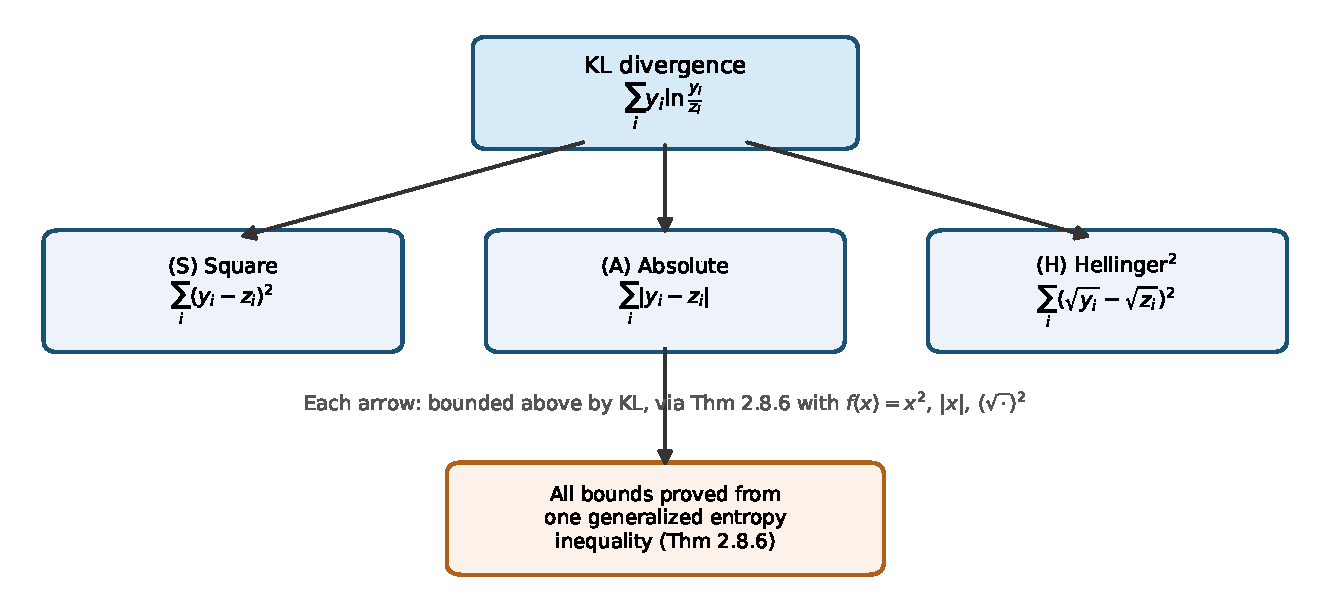
\includegraphics[width=0.62\textwidth]{distance_hierarchy}
  \end{center}
\end{frame}

% ============================================================
\begin{frame}{Proof of Corollary 2.8.8}
  \textbf{Proof.} Taking Theorem 2.8.6 and substituting $f(x)=x^2$ or
  $f(x)=|x|$ directly gives (S) or (A) respectively.

  To prove (H), for $t,y,z>0$ define
  \[
    g(t) := -\ln(t) + t - 1 \;\ge\; 0
  \]
  \textbf{Plain English.} $g(t)$ measures how far $t$ is from $1$ in a
  logarithmic sense; it is a standard fact that $g(t)\ge0$ for all $t>0$,
  with equality only at $t=1$ (this is essentially Gibbs' inequality again).

  This implies (after some algebra)
  \[
    f(y,z) \;:=\; y\ln\frac{y}{z} - (\sqrt{y}-\sqrt{z})^2 + z - y
    \;=\; 2y\,g(\sqrt{z/y}) \;\ge\; 0,
  \]
  hence $y\ln(y/z) - (\sqrt{y}-\sqrt{z})^2 \ge y - z$. Summing over
  $i=1,\ldots,d$ (with $y=y_i$, $z=z_i$),
  \[
    \sum_i y_i\ln\frac{y_i}{z_i} - \sum_i(\sqrt{y_i}-\sqrt{z_i})^2
    \;\ge\; \sum_i y_i - \sum_i z_i \;\ge\; 1 - 1 \;=\; 0,
  \]
  from which (H) follows (using $\sum_i z_i \le 1$). $\blacksquare$
\end{frame}

% ============================================================
\begin{frame}[fragile]{Python: Verifying the Entropy Inequalities Numerically}
  We numerically check Corollary 2.8.8 for a concrete pair of distributions
  $y=(0.5, 0.3, 0.2)$ and $z=(0.3, 0.4, 0.3)$ (both probability vectors on
  $3$ outcomes).

\begin{lstlisting}
import numpy as np

y = np.array([0.5, 0.3, 0.2])
z = np.array([0.3, 0.4, 0.3])

kl = np.sum(y * np.log(y / z))                       # KL(y || z)
square    = np.sum((y - z)**2)                        # (S)
absolute  = np.sum(np.abs(y - z))                      # (A)
hellinger = np.sum((np.sqrt(y) - np.sqrt(z))**2)       # (H)

print(f"KL={kl:.4f}  square={square:.4f}  absolute={absolute:.4f}  hellinger2={hellinger:.4f}")
# KL=0.0880  square=0.0600  absolute=0.4000  hellinger2=0.0427
\end{lstlisting}

  \textbf{Reading the output.} All three bounds hold ($0.0600\le0.0880$,
  $0.4000\le\sqrt{2\cdot0.0880}=0.4196$, $0.0427\le0.0880$), exactly as
  Corollary 2.8.8 guarantees.
\end{frame}

% ============================================================
\begin{frame}{Entropy Inequalities: Actual Distance vs.\ KL-Based Bound}
  \begin{center}
    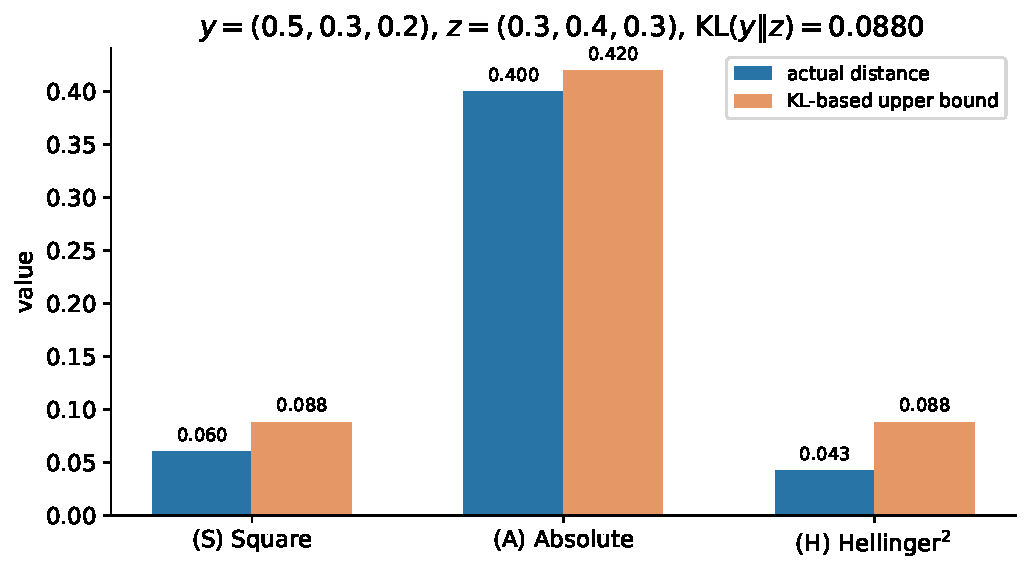
\includegraphics[width=0.62\textwidth]{entropy_verify}
  \end{center}
\end{frame}

\section{2.8.2 Dealing with Semimeasures}

% ============================================================
\begin{frame}{Why Semimeasures Are a Headache}
  Recall (Definition 2.2.11) that a \emph{semimeasure} $\nu$ relaxes a
  probability measure by allowing $\sum_{a} \nu(\Gamma_{xa}) \le \nu(\Gamma_x)$
  rather than requiring equality: some probability mass can simply be
  ``missing''.

  \textbf{The problem.} Measure theory itself is already a mature,
  well-developed field. Semimeasure theory, by contrast, essentially does
  not exist as a developed field --- yet semimeasures are exactly what
  Solomonoff induction and the AIXI agent are built on (via lower
  semicomputable semimeasures, class $\mathcal{M}_{sol}$). This subsection
  lists several pragmatic workarounds used throughout the book, since a full
  semimeasure theory is beyond its scope.

  \begin{block}{Only use $\nu$ on cylinder sets}
    For most of the book we only ever need to know $\nu$ on \emph{cylinder
    sets} $\Gamma_x$ (the set of all infinite sequences starting with the
    finite string $x$). The most frequently used quantity is the predictive
    distribution
    \[
      \nu(x_t \mid x_{<t}) \;\equiv\; \nu(\Gamma_{x_{1:t}}) / \nu(\Gamma_{x_{<t}}).
    \]
    \textbf{Plain English.} This is simply ``the probability of the next
    symbol given everything seen so far'', written as a ratio of two
    cylinder-set masses. For predictions over a fixed finite lifetime $m$,
    the sample space is finite and this trivializes semimeasure theory
    entirely.
  \end{block}
\end{frame}

% ============================================================
\begin{frame}{Developing or Deriving Semimeasure Results}
  \begin{block}{Develop semimeasure theory}
    Extending measure theory's definitions and results to semimeasures could
    be an interesting research program, but is beyond the book's scope
    (left as an exercise for ``eager math students'').
  \end{block}

  \begin{block}{Derive required semimeasure results}
    A more focused alternative: only develop what is actually needed for
    this book. Even this is a major undertaking. Extending \emph{finitary}
    results (e.g.\ the entropy inequalities of Corollary 2.8.8) is often not
    too hard and has been done. For others --- such as martingale
    convergence, or even the general definition of expectation --- one would
    need to dig much deeper.
  \end{block}

  \begin{block}{Defining $\nu$ on measurable sets}
    Strictly, $\nu$ is only a \emph{pre}-semimeasure. To extend it to a full
    $\sigma$-algebra $\mathcal{F}$ we would need a semimeasure version of
    Carathéodory's extension theorem. The book sketches (but does not fully
    verify) a candidate construction using an \emph{inner} semimeasure
    $\nu_*(A) := \sup_{\mathcal{S}:\Gamma_\mathcal{S}\subseteq A}
    \sum_{x\in\mathcal{S}} \nu(\Gamma_x)$ and an \emph{outer} semimeasure
    $\nu^*(A) := \inf_{\mathcal{S}\supseteq A} \sum_{x\in\mathcal{S}'}
    \nu(\Gamma_x)$, noting this remains a genuinely open research problem.
  \end{block}
\end{frame}

% ============================================================
\begin{frame}{Expectations With Respect to Semimeasures}
  Once we can evaluate $\nu$ on measurable sets, we could (mis)use the
  general definition of expectation for non-negative $f$:
  \[
    \E_\nu[f] \;:=\; \int_0^\infty f^*(t)\,dt \qquad \text{with} \qquad
    f^*(s) := \nu(\{\omega\in\Omega : f(\omega) > s\}).
  \]
  \textbf{Plain English.} This is the standard ``layer-cake'' formula for
  expectation: integrate, over all thresholds $s$, the probability that $f$
  exceeds $s$.

  \textbf{The catch: linearity breaks.} Decomposing the constant function
  $1 = \sum_{a\in\mathcal{X}} f_a$ with $f_a(x_{1:\infty}) := [\![x_1=a]\!]$
  (an indicator that the first symbol is $a$), we get
  \[
    \E\Big[\sum_a f_a\Big] \;=\; \E_\nu[1] \;=\; \nu(\Gamma_\epsilon)
    \;\ge\; \sum_{a\in\mathcal{X}} \nu(\Gamma_a) \;=\; \sum_a \E[[\![x_1=a]\!]]
    \;=\; \sum_a \E[f_a].
  \]
  \textbf{Plain English.} $\Gamma_\epsilon$ is the cylinder set for the empty
  string (the whole sample space). Because $\nu$ can leak mass, the
  expectation of a sum of indicators can strictly exceed the sum of their
  individual expectations --- i.e.\ \textbf{expectation is no longer
  linear} once $\nu$ is only a semimeasure. Other definitions of $\E$ may
  preserve linearity, at the cost of other properties.
\end{frame}

% ============================================================
\begin{frame}{Include Finite Sequences: Modeling ``Death''}
  Some monotone Turing machines may not output infinite sequences, but stop
  or loop forever after only a finite output. The most honest fix: enlarge
  the sample space from $\mathcal{X}^\infty$ to $\mathcal{X}^\infty \cup
  \mathcal{X}^*$, and convert any semimeasure $\nu$ into a genuine measure
  $\tilde\nu$ via
  \[
    \tilde\nu(\Gamma_x^*) := \nu(\Gamma_x) \qquad \text{and} \qquad
    \tilde\nu(\{x\}) := \nu(\Gamma_x) - \sum_{a\in\mathcal{X}} \nu(\Gamma_{xa}).
  \]
  \textbf{Plain English.} $\Gamma_x^*$ is the cylinder set extended to also
  include the finite string $x$ itself. $\tilde\nu(\{x\})$ --- the
  ``missing'' probability mass at $x$ --- is interpreted as the probability
  that the source (the world, or the predictor/agent) \emph{dies} exactly
  after emitting $x$. This is used later in Section 15.7. Because
  $\Gamma_x^* = \{x\} \cup \bigcup_a \Gamma_{xa}^*$, indeed
  $\tilde\nu(\Gamma_x^*) = \tilde\nu(\{x\}) + \sum_a \tilde\nu(\Gamma_{xa}^*)$
  --- so $\tilde\nu$ is a genuinely proper (non-leaky) probability measure.
\end{frame}

% ============================================================
\begin{frame}{Where the Missing Mass Goes}
  \begin{center}
    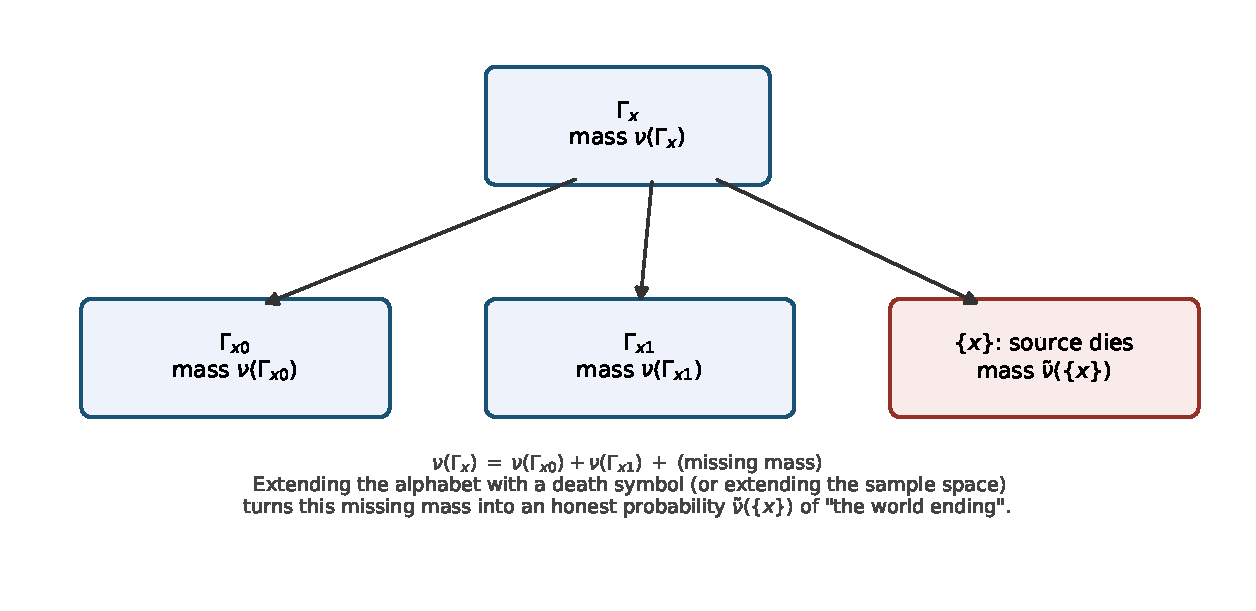
\includegraphics[width=0.6\textwidth]{semimeasure_leak}
  \end{center}
\end{frame}

% ============================================================
\begin{frame}{Extending the Alphabet With a Death Symbol}
  A similarly ``honest'' idea: extend the alphabet to
  $\mathcal{X} \cup \{\bot\}$, adding a special ``death'' symbol $\bot$
  (pronounced ``bottom''), and extend $\mu$ via
  \[
    \nu(\Gamma_{x\bot^k}) := \nu(\Gamma_x) - \sum_{a\in\mathcal{X}} \nu(\Gamma_{xa})
    \quad \forall k\in\mathbb{N}^+, \qquad
    \nu(\Gamma_{x\bot y}) := 0 \quad \forall y \in (\mathcal{X}\cup\{\bot\})^*\setminus\{\bot\}^*.
  \]
  \textbf{Plain English.} Once $\bot$ has occurred, it just keeps recurring
  forever (the world has ``ended''); no other symbol can follow it. This
  keeps the convenience of working with proper infinite sequences (no need
  for the hybrid finite/infinite sample space above), while $\nu$ becomes a
  genuine measure on $(\mathcal{X}\cup\{\bot\})^\infty$.

  \textbf{Consequence for agents.} If we assign reward $0$ once $\bot$ is
  observed, the Bellman equations (used to define optimal value functions)
  remain valid, and agent death is faithfully modeled. One caveat: some
  results have only been derived for binary $\mathcal{X}$, so are not
  available once $\bot$ is added to a binary alphabet (making it
  effectively ternary).
\end{frame}

% ============================================================
\begin{frame}{Solomonoff Normalization}
  \begin{block}{Solomonoff normalization}
    Given a semimeasure $\nu$ on cylinder sets, define
    \[
      \nu_{norm}(x_t\mid x_{<t}) := \frac{\nu(\Gamma_{x_{1:t}})}{\sum_{x_t\in\mathcal{X}} \nu(\Gamma_{x_{1:t}})},
      \quad
      \nu_{norm}(\Gamma_{x_{1:n}}) := \prod_{t=1}^n \nu_{norm}(x_t\mid x_{<t}),
      \quad \nu_{norm}(\epsilon):=1.
    \]
  \end{block}
  \textbf{Plain English.} At every step, we simply rescale (renormalize)
  the semimeasure's predictive probabilities so they sum to exactly $1$,
  then multiply these normalized one-step probabilities together. This
  gives a properly normalized probability measure that still
  \emph{dominates} $\nu$ (i.e.\ $\nu_{norm}(\Gamma_x)\ge\nu(\Gamma_x)$),
  which is the key property needed later (Proposition 3.1.4). Downsides:
  $\nu_{norm}$ is no longer lower semicomputable (only limit-computable),
  even if $\nu$ was, and we lose the ``semimeasure defect'' that used to
  be attributed to death of an agent.
\end{frame}

% ============================================================
\begin{frame}{Lower-Limit Normalization}
  \begin{block}{Lower limit normalization}
    We could instead look for the \emph{largest measure} $\underline\nu \le
    \nu$. This is unique, and can be represented [Hut14b] as
    \[
      \underline\nu(\Gamma_{x_{<t}}) := \lim_{n\to\infty}
      \sum_{x_{t:n}} \nu(\Gamma_{x_{1:n}}).
    \]
  \end{block}
  \textbf{Plain English.} We push all remaining probability mass as far
  into the future as possible before ``giving up'' on it, and take the
  limit. The limit exists because the sum is decreasing in $n$ (a
  consequence of $\nu$ being a semimeasure): $\underline\nu$ is the
  ``most pessimistic'' proper measure consistent with never assigning more
  mass than $\nu$ itself does.
\end{frame}

% ============================================================
\begin{frame}[fragile]{Python: A Concrete Semimeasure That Is Not a Measure}
  The book gives a small concrete example (p.\ 114): a semimeasure $\nu$
  with $\nu(\Gamma_{1^n}) = 1/2$ for all $n\ge1$, $\nu(\Gamma_{0^n}) =
  2^{-n-1}$, and $\nu = 0$ on every other sequence prefix.

\begin{lstlisting}
import numpy as np

n_max = 6
nu_1n = np.array([0.5] * n_max)                 # nu(Gamma_{1^n}), n=1..n_max
nu_0n = np.array([2.0**(-n-1) for n in range(1, n_max+1)])  # nu(Gamma_{0^n})

print("nu(Gamma_{1^n}):", nu_1n)
print("nu(Gamma_{0^n}):", nu_0n)

# nu(Gamma_0) = 1/4 directly, but the LARGEST MEASURE below nu (underline_nu)
# assigns underline_nu(0) = lim_{n->inf} nu(Gamma_{0^n}) = 0
print("nu(0)=0.25  underline_nu(0)=0.0  underline_nu(eps)=0.5")
\end{lstlisting}

  \textbf{Plain English.} Even though $\nu$ assigns positive mass $1/4$ to
  ``starts with 0'', that mass keeps shrinking geometrically the longer the
  run of 0s must continue, all the way down to $0$ in the limit. So the
  lower-limit-normalized measure $\underline\nu$ (which looks arbitrarily
  far into the future) assigns $0$ to that same cylinder set --- illustrating
  $\underline\nu \ne \nu$ in general, and that $\underline\nu$ is not itself
  a probability measure ($\underline\nu(\Gamma_\epsilon)=1/2\ne1$) until
  renormalized.
\end{frame}

% ============================================================
\begin{frame}{A Semimeasure That Is Not a Measure: The Plot}
  \begin{center}
    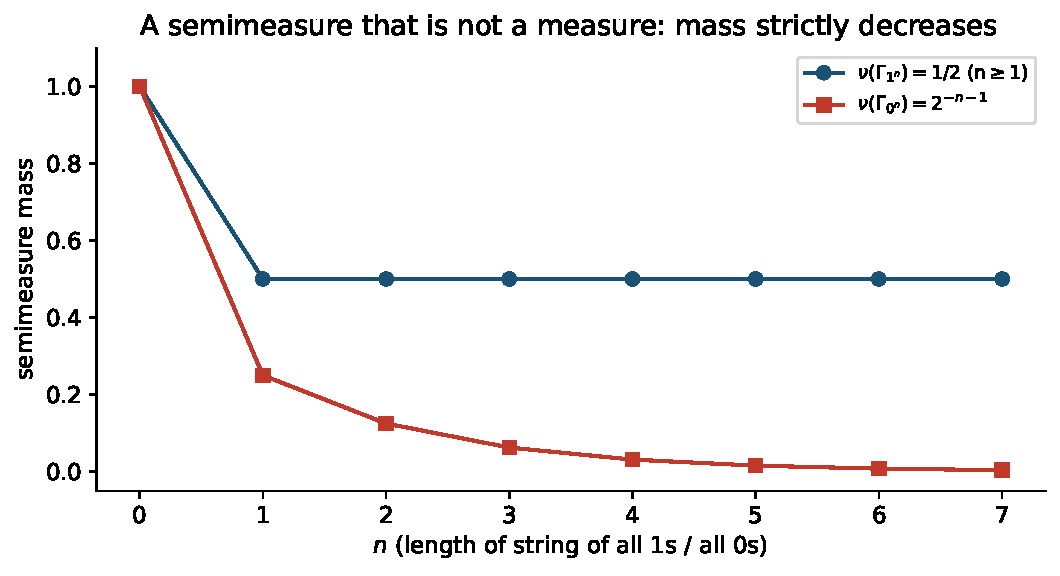
\includegraphics[width=0.55\textwidth]{solomonoff_norm}
  \end{center}
\end{frame}

% ============================================================
\begin{frame}[allowframebreaks]{Restricted Classes of Measures}
  \textbf{Computable measures $\mathcal{M}_{comp}$.} A monotone Turing
  machine that is \emph{guaranteed} to output only infinite sequences
  generates a properly normalized probability measure. Let
  $\mathcal{M}_{comp}$ be the class of all such measures. Each measure in
  $\mathcal{M}_{comp}$ is computable, but --- unlike $\mathcal{M}_{sol}$,
  the class of lower semicomputable semimeasures --- $\mathcal{M}_{comp}$ is
  not effectively enumerable, hence not approximable by an algorithm that
  lists it out.

  \textbf{Global assumption: $\mu$ is a proper probability measure.} This is
  assumed throughout the rest of the book. Some key theorems (such as the
  entropy inequalities, Corollary 2.8.8) genuinely fail if the true
  environment $\mu$ is only a semimeasure. There is generally no pressing
  need to model semimeasure environments directly, except possibly to model
  finite universes or death.

  \framebreak

  \textbf{Primitive recursive measures $\mathcal{M}_{pr}$.} Instead of
  considering all Turing machines, restrict to \emph{primitive recursive}
  (p.r.) functions --- total functions with a primitive-recursive upper
  bound on their own run-time. This class contains virtually every
  computable function one usually encounters in practice; functions that
  are computable but not p.r.\ are extremely slow-growing (e.g.\ functions
  growing like the Ackermann function). The class of p.r.\ functions is
  itself recursively enumerable [Liu60], so it can be converted into an
  enumeration of p.r.\ measures $\mathcal{M}_{pr}\subset\mathcal{M}_{comp}$,
  e.g.\ via Solomonoff normalization. Assuming a computable prior weight
  $w_\nu$, the Bayesian mixture $\xi$ over $\mathcal{M}_{pr}$ is then
  computable --- but, perhaps surprisingly, $\xi\notin\mathcal{M}_{pr}$
  itself (mixing takes you outside the class you started with).

  \textbf{Reflective-oracle computable measures $\mathcal{M}_r^O$.} In
  Section 10.5 we will meet a strictly larger class
  $\mathcal{M}_r^O \supset \mathcal{M}_{comp}$ of measures computable with
  the help of a \emph{reflective oracle}. It has the remarkable property
  that the normalized Bayes mixture both dominates the class \emph{and} is
  itself a member of the class; even the Bayes-optimal policy
  $\pi_\xi^*$ is in the class, solving the long-standing \emph{Grain of
  Truth problem} (the question of whether an agent's own prior belief class
  can contain the true environment together with rational agents reasoning
  about each other).
\end{frame}

% ============================================================
\begin{frame}{Conclusion of Section 2.8.2}
  Ideally, the \emph{entire} book would be developed for semimeasures,
  since $\mathcal{M}_{sol}$ (lower semicomputable semimeasures) is the core
  class of interest for Solomonoff induction and the AIXI agent. But this is
  unfortunately not feasible with current mathematical tools. As a
  consequence, most of the theory in this book is developed for proper
  measures only, and the workarounds above are applied whenever
  semimeasures unavoidably crop up.

  \textbf{Rule of thumb, if in doubt.} Assume the death symbol $\bot$ has
  been added to the alphabet $\mathcal{X}$ (and, in the agent case, assume
  reward $r=0$ once $\bot$ is perceived), or simply restrict attention to
  $\mathcal{M}_{pr}$ or $\mathcal{M}_{comp}$ instead of the full
  $\mathcal{M}_{sol}$.
\end{frame}

\section{2.8.3 Probability Zero}

% ============================================================
\begin{frame}{Why Probability-Zero Events Matter}
  For continuous sample spaces $\Omega$, probability-zero events are
  everywhere. Example: throwing darts at a dartboard --- the probability of
  hitting any single, specific point is exactly zero, even though every
  player's dart lands \emph{somewhere}, so some probability-zero outcome
  always occurs. Technically this is modeled using a probability
  \emph{density} rather than a probability mass. Conditional probabilities
  and expectations conditioned on probability-zero outcomes can still be
  defined, but require care.

  \textbf{Good news for this book.} Nearly all of the book deals only with
  \emph{discrete} random variables, which simplifies matters considerably
  --- but does not entirely trivialize the problem, as we will see. This
  subsection collects the relevant issues and the (single) convention
  adopted throughout the rest of the book, so as not to clutter later
  chapters with repeated caveats.
\end{frame}

% ============================================================
\begin{frame}{Expectation for Partial Functions}
  Recall the definition of expectation (Definition 2.2.36) works cleanly as
  long as the function $g$ is \emph{total}. If $g$ can take infinite values,
  or is only \emph{partial} (undefined on some inputs), the correct
  definition for discrete $X$ is
  \[
    \E[g(X)] \;=\; \sum_{x\in X(\Omega): p(x)>0} g(x)\,p(x)
    \qquad \text{for } g: \mathbb{R}\to\mathbb{R}\cup\{\pm\infty\}\cup\{\bot\}.
  \]
  \textbf{Plain English.} We simply skip any outcome $x$ that has zero
  probability $p(x)=0$ before summing --- so it never matters whether $g(x)$
  is well-defined there. For total, finite-valued $g$ this restriction is
  redundant and can be dropped, but we still want $\E$ to be defined even
  when $g$ is infinite or undefined ($\bot$) at some zero-probability point.

  \textbf{Worked example.} Let $\Omega=\{0,1\}$ and $g(x):=1/p(x)$. If
  $\forall x.\,p(x)>0$, then $\E[g(X)] = \sum_{x\in\Omega} 1 = 2$. But if
  $p(0)=0$ (so $g(0)$ is undefined, dividing by zero), we simply get
  $\E[g(X)] = g(1)p(1) = 1$: the problematic point $x=0$ is silently
  excluded from the sum because it has probability zero.
\end{frame}

% ============================================================
\begin{frame}{Conditioning on Probability-Zero Events}
  \begin{block}{Conditioning on $P(A)=0$}
    Since a probability-zero event will (almost) never occur, the
    \emph{safest} option is to simply leave $P(B\mid A)$ \textbf{undefined}
    whenever $P(A)=0$. But this is restrictive (it does not allow
    conditional \emph{densities}, needed in continuous settings) and
    cumbersome (it requires special-casing every theorem). There is no
    fully satisfactory general solution to this problem; see [Hut05b,
    Sec.\ 3.9.1] for some unorthodox suggestions.
  \end{block}

  \begin{block}{Conditioning on $\mu(x_{<t})=0$: the convention used here}
    We only encounter this issue for random sequences and $\mu(\cdot\mid
    x_{<t})$ when $\mu(x_{<t})=0$, so we focus on this one special case.
    \textbf{The adopted convention:} add the qualifier ``holds with
    $\mu$-probability $1$'' to every theorem statement, if it is not there
    already. Since $\mu(x_{<t})=0$ is itself a probability-zero event, we
    are then free to \emph{safely ignore} such histories $x_{<t}$
    altogether when checking whether a theorem's conclusion holds.
  \end{block}
\end{frame}

% ============================================================
\begin{frame}{Probability Kernels}
  In the agent setting, we consider a policy $\pi$ interacting with an
  environment $\mu$, generating a history $h_{1:\infty}$. We sometimes need
  to know how a policy $\pi$ \emph{would} continue a history $h_{<t}$ even
  if $h_{<t}$ itself has probability $0$ under $\pi$ (e.g.\ because
  $h_{<t}$ was actually generated by a \emph{different} policy).

  \textbf{The solution: probability kernels.} Start with \emph{conditional}
  distributions directly, and take their product. Formally, a
  \emph{probability kernel} is a family of functions
  $\mu_t: \mathcal{X}^t \to \Delta\mathcal{X}$ for each $t\in\mathbb{N}$,
  where for every history $x_{<t}$, $\mu_t(\cdot\,;x_{<t})$ is a genuine
  probability distribution over the next symbol $\mathcal{X}$ (note the
  semicolon --- it is not the same as a conditional probability derived
  \emph{from} a joint measure).
  \[
    \mu(x_{1:n}) := \prod_{t=1}^n \mu_t(x_t; x_{<t})
    \qquad \text{and} \qquad
    \mu(x_t\mid x_{<t}) := \mu_t(x_t; x_{<t}).
  \]
  \textbf{Plain English.} This product defines a genuine joint measure
  $\mu$, and the conditional $\mu(x_t\mid x_{<t})$ is \emph{uniquely and
  well-defined even when $\mu(x_{<t})=0$} --- because we started from the
  conditionals themselves rather than trying to derive them via division.
  The collection of kernels $(\mu_t)$ therefore carries strictly \emph{more}
  information than the joint measure $\mu$ alone.
\end{frame}

% ============================================================
\begin{frame}{Probabilistic Turing Machines and Kernels}
  Consider a probabilistic Turing machine $T$ that lower semicomputes
  semiprobability kernels, i.e.\ $\nu_T(x_t\mid x_{<t})$ is the probability
  that $T(x_{<t},t,\text{random noise})$ outputs $x_t$.

  \textbf{A subtly smaller class.} The class $\{\nu_T : T \text{ a TM}\}$ is
  recursively enumerable, and contains \emph{all and only} the semimeasures
  that are \emph{conditionally} lower semicomputable. This class is
  ``slightly'' smaller than $\mathcal{M}_{sol}$, since a semimeasure
  $\nu\in\mathcal{M}_{sol}$ is not automatically \emph{conditionally} lower
  semicomputable.

  \begin{block}{Pragmatic approach (used throughout the book)}
    Take the approach above, but without being pedantic about the semicolon
    notation and the time index $t$: simply write $\nu(x_t\mid x_{<t})$
    directly, even though strictly speaking it is a probability kernel and
    not literally a conditional distribution when $\nu(x_{<t})=0$.
  \end{block}

  \textbf{Worked example.} If $\nu_T^s(x_{<t})$ (for $s=1,2,3,\ldots$) is a
  lower-computation sequence approximating $\nu_T(x_{<t})$ from below,
  define $\nu_T^s(x_t\mid x_{<t}) := 1/|\mathcal{X}|$ (or any other
  computable placeholder) as long as $\nu_T^s(x_{<t})=0$. Once (if ever)
  $\nu_T^s(x_{<t})>0$, switch to $\nu_T^s(x_t\mid x_{<t}) :=
  \nu_T^s(x_{1:t})/\nu_T^s(x_{<t})$. Note the resulting conditional
  distribution is generally \emph{not} lower semicomputable, but only
  \emph{limit-computable} in every case.
\end{frame}

% ============================================================
\begin{frame}{2.8.4 Exercises (Section 2.8)}
  The book poses seven exercises testing the material of Section 2.8:
  \begin{enumerate}
    \item Prove the Absolute distance and the Un-Squared Hellinger distance
      $\sqrt{H}$ are both metrics, but the KL divergence is not.
    \item Show the bounds in Corollary 2.8.8 are tight: the ratio of
      left-hand side to right-hand side can get arbitrarily close to $1$.
    \item Generalize all distance definitions and bounds to probability
      measures on general sample spaces $\Omega$, except for the $2$-norm;
      explain what goes wrong for the $2$-norm.
    \item Derive an explicit expression for $\tilde\nu(\Gamma_x)$ (note:
      $\Gamma_x\ne\Gamma_x^*$) and show $\underline\nu(\Gamma_{x<t}) =
      \tilde\nu(\Gamma_{x<t})$, both defined in Section 2.8.2.
    \item Prove all claims made in Section 2.8.2.
    \item[6--7.] (Open-ended, research-level) Suitably generalize all
      results in this book to semimeasures, or extend a measure-theory
      textbook's definitions and results to semimeasures, and prove them.
  \end{enumerate}
\end{frame}

\section{2.9 History and References: Overview}

% ============================================================
\begin{frame}{Purpose of This Section}
  Section 2.9 is the book's guide to the wider literature behind every topic
  covered in Chapter 2. It is organized to mirror the chapter's own
  subsections (2.1 through 2.8), giving, for each, the key historical
  breakthroughs and the standard textbooks/papers a reader could turn to for
  more depth.

  \textbf{Two anchor references for AI in general.}
  \begin{itemize}
    \item \emph{Artificial Intelligence: A Modern Approach} [RN20] --- the
      canonical AI textbook, comprehensive overview with over a thousand
      further AI-related references.
    \item \emph{An Introduction to Kolmogorov Complexity and Its
      Applications} [LV19] --- its introductory chapter covers similar
      background material, with many further related references.
  \end{itemize}
  This history section itself is an updated version of an earlier one from
  the author's PhD-thesis-turned-monograph [Hut05b, Sec.\ 2.5].
\end{frame}

% ============================================================
\begin{frame}{A Timeline of Selected Milestones}
  \begin{center}
    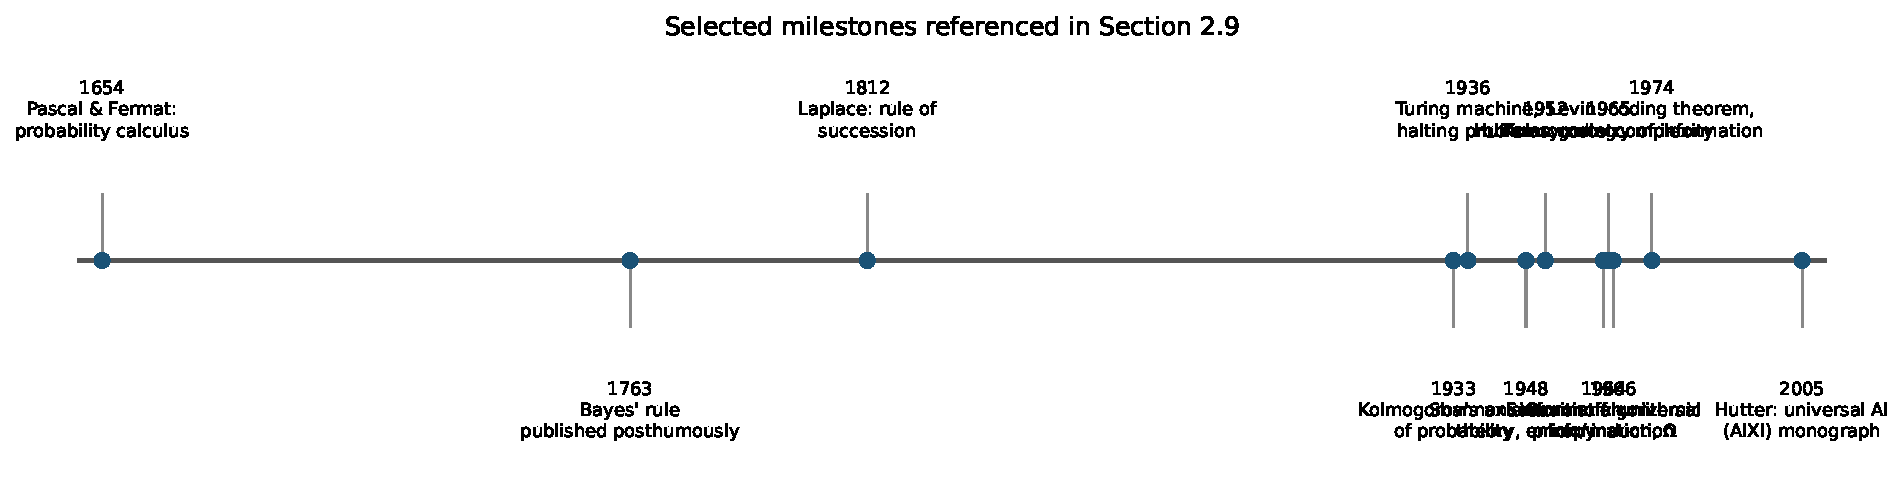
\includegraphics[width=0.98\textwidth]{timeline}
  \end{center}
\end{frame}

\section{Histories by Subsection (2.1--2.4)}

% ============================================================
\begin{frame}{2.1 Binary Strings \& 2.2 Measure Theory and Probability}
  \textbf{Binary strings (2.1).} Based on the corresponding sections in
  [Hut05b] and [LV19]. \emph{Principles of Mathematical Analysis} by Rudin
  [RT64] gives an introduction to the real-analysis concepts assumed
  throughout. Prefix codes are discussed in depth in Li and Vitányi's book
  [LV19]; the general theory of coding and prefix codes is covered in
  [Gal68].

  \textbf{Measure theory and probability (2.2).} Based on material from
  [GS20]. \emph{Real Analysis} by Stein and Shakarchi [SS09] gives a slower,
  more formal treatment of measure theory. The i.i.d.\ assumption is
  prevalent in statistics and machine learning, but unsuitable for AGI
  [hut22].

  \textbf{A brief history of probability.} Games of chance date back to
  around 300 B.C., but the first \emph{mathematical analysis} of
  probability appears much later. Key breakthroughs, chronologically: a
  systematic way of calculating probabilities by Cardano [Car63]; a
  systematic treatment via Pascal (in correspondence with Fermat) and
  conditional probability [Pas54]; Bayes' rule [Bay63]; the distinction
  between subjective and objective probability, and the weak law of large
  numbers, by Bernoulli [Ber13]; equi-probability due to symmetry by Laplace
  [Lap12]; the principle of indifference by Keynes [Key21]; Kolmogorov's
  axioms of probability theory [Kol33]; early attempts to define randomness
  of individual sequences by von Mises [Mis19], Wald [Wal37], and Church
  [Chu40], finally made successful by Martin-Löf [ML66]; and the notion of a
  universal a priori probability by Solomonoff [Sol64], mathematically
  investigated by Levin [ZL70a, Lev74].
\end{frame}

% ============================================================
\begin{frame}{Recommended Probability Textbooks and Statistical Inference (2.3)}
  \textbf{Textbooks for probability theory.} \emph{Probability and Random
  Processes} by Grimmett et al.\ [GS20] is a gentle introduction with
  plenty of exercises (the basis for most of this chapter). \emph{Introduction
  to Probability Models} by Ross [Ros14] is more advanced, with a similar
  structure but going well beyond this book's scope. For the early history
  of probability, see Hacking [Hac75] and Hald [Hal90]; for the 20th-century
  foundations, see Schnorr [Sch71] and the PhD theses of van Lambalgen
  [Lam87] and Wang [Wan96]. See also Shafer \& Vovk [SV01] for a
  game-theoretic/finance perspective, and Feller [Fel68] as a standard
  textbook. A philosophical treatise on conditional probability is [Haj11].

  \textbf{Statistical inference and estimation (2.3).} A great introduction
  to frequentist statistics, focusing on general theory over specific
  models, is Wasserman [Was10]. Section 2.3.4 is based on a chapter from
  \emph{Elements of Information Theory} [CT06], where the Cramér--Rao
  inequality (Theorem 2.3.14) is proven; the ``sunrise problem'' was first
  described by Laplace [Lap40], where the rule of succession now known as
  \emph{Laplace's Rule} was introduced (Section 2.4.3).
\end{frame}

% ============================================================
\begin{frame}[allowframebreaks]{2.4 Bayesian Probability Theory}
  The limitations of frequentist statistics are discussed in [Hut05b,
  Sec.\ 2.3.1][Háj09b]: the naive definition is \emph{circular} (though see
  Cournot's forgotten principle [Cou43]); identical events are a mirage
  (the \emph{reference class problem}); and the most serious limitation is
  the assumption of i.i.d.\ data.

  \textbf{Alternatives to Bayesian reasoning in AI's history.} Default
  reasoning [Rei80]; non-monotonic logic [MD80]; circumscription [McC80];
  certainty factors [Sho76, BS84]; Dempster--Shafer theory [Dem68, Sha76];
  fuzzy logic [Zad65, Zim91]; possibility theory [Zad78]; imprecise
  probabilities [Wal91, Hut03f, ZH05, PZTH07, Hut09h, PZTH09]; robust
  Bayesian analysis [RIR00]; and many others (see [Fin73, Wal91, RN20] for a
  more detailed account).

  \framebreak

  \textbf{Why classical probability theory fell briefly out of favor, and
  its return.} Many reasons were put forward in the 1970s: strict numerical
  values seemed inappropriate for qualitative reasoning, probability theory
  cannot deal with impreciseness/vagueness/subjective belief, or is just
  impractical. But all these alternative approaches turned out to have
  \emph{their own} problems --- unclear semantics, lack of self-consistency,
  or failure to scale. Bayesian and frequentist probability theory leave the
  fewest open questions, especially Bayesianism, with solid justifications
  via Cox's axioms [Cox46] and Dutch book arguments [Háj09a, Pre09, Sec.\ 2].
  The debates [Che85, Che88] have essentially settled in the new millennium
  in favor of machine-learning systems based on classical statistics
  [HTF09] and increasingly (sometimes robust) Bayesian methods [Bis06,
  KF10, Mur22, Mur23] --- returning to its roots of 1763 [Bay63].

  \framebreak

  \textbf{Bayes' Law and Laplace's Rule.} Bayes' Law is one of the earliest
  non-trivial rules in probability and statistics [Bay63], which
  \emph{Laplace's Rule} [Lap40] builds upon. Jaynes' philosophical text
  [Jay03] treats probability theory as a natural extension of (Boolean)
  logical reasoning; Earman [Ear93] is another philosophical text on Bayes;
  Gelman [GCSR95] is more practical (data analysis); Berger [Ber93] sits
  in-between. More on Bayesian inference and choices of model class/prior:
  [BC16, GvdV17]; standard Bayesian machine-learning textbooks: [Bis06,
  Mur22, Mur23].

  \framebreak

  \textbf{Objective vs.\ subjective probability.} An ongoing debate,
  sharpened in the 20th century. Advocates of the relative-frequency /
  objective interpretation: Kolmogorov [Kol63], Fisher [Fis22], von Mises
  [Mis28]. Hajek [Háj96, Háj09b] offers fifteen arguments against
  finite/hypothetical frequentism. Advocates of probability as degrees of
  belief: Popper [Pop34], Ramsey [Ram31], Finetti [Fin37, Fin74], Cox
  [Cox46], Savage [Sav54], Jeffreys [Jef83], Good [Gol06]. See [OBD+06,
  O'H19] on eliciting subjective probabilities from experts; objective
  priors are advocated in [Ber06, BBS24], and ``universal priors'' in
  [Hut07e, RH11]. Jeffreys' objective prior (Definition 2.4.11) and its
  reparameterization invariance is discussed further in [Pre09, O'H10,
  Lee12]. See [Goo71] for a classification of ``46656 varieties of
  Bayesians'', and [Pre09, Sec.\ 2] for an overview of justifications of the
  Kolmogorov axioms from various perspectives.

  \framebreak

  \textbf{Inductive logic and the reference class problem.} Carnap [Car48,
  Car50] tried to supplement logic with probability theory, giving
  so-called \emph{inductive logic}. This works for propositional logic
  [Jay03], but extending it satisfactorily to predicate logic failed for a
  long time [Put63], until finally solved [GS82, HLNU13b, HLNU13a,
  GBTC+20]. The closely related \emph{reference class problem} is addressed
  in [Rei49, Kyb77, Kyb83, BGHK92].
\end{frame}

\section{Histories by Subsection (2.5--2.7)}

% ============================================================
\begin{frame}[allowframebreaks]{2.5 Information Theory and Coding}
  This section is based on the texts [Mac03, CT06, JJHH03, LV19]. The
  entire discipline of information theory originates from Shannon's
  original paper [Sha48], formalizing the problem of transmitting a message
  over a noisy communication medium, and introducing entropy while proving
  the source-coding theorem (Theorem 2.5.22).

  \textbf{Estimating and predicting entropy.} The entropy of English text
  has been estimated through experiments using both humans [Sha51] and
  algorithms [Gue09, CK78] as predictors. The Kraft inequality is due to
  Kraft [Kra49]. The Kullback--Leibler divergence originates in a paper by
  the eponymous pair [KL51].

  \framebreak

  \textbf{Coding methods.} Shannon--Fano coding refers to two similar coding
  methods, by Shannon [Sha48] and Fano [Fan49]. Huffman coding [Huf52] is
  provably optimal given each symbol coded individually with a known
  frequency distribution. Better results come from block codes such as
  arithmetic codes [Pas76, HV91], which outperform Huffman coding on
  low-entropy messages. Golomb codes [GVV75] are optimal when symbols follow
  a geometric distribution. Pre-coding transformations like \emph{run length
  encoding} [RC67] or \emph{move-to-front} [Rya80], or the Burrows--Wheeler
  transform [BW94], can be applied before a further code to shrink the
  message more.

  \framebreak

  \textbf{Dictionary and mixture-based compressors.} Dictionary coders
  compress by replacing a substring with an index into a lookup table: the
  Lempel--Ziv family starts with LZ77 [ZL77] and LZ78 [ZL78], popularizing
  this technique and extending to LZW [Wel84], LZRW [Wil91b], and LZSS
  [SS82]. \emph{Context mixing compressors} are similar to Context Tree
  Weighting (covered in Chapter 4): they estimate a probability
  distribution as a mixture of models and compress with respect to it using
  arithmetic coding [Sai04]. The PAQ family [Mah05] takes a weighted average
  of models; later improved using a neural network for the mixture [Mah07].

  \framebreak

  \textbf{Surveys and the Hutter Prize.} A survey of compression techniques,
  with trade-offs between compression time, compression ratio, and
  decompression time, is given in [Mah12, SM10]; further comparisons in
  [Mah22, Nem22]. The \textbf{Hutter Prize} [Hut20a] offers a monetary
  reward for compressing \texttt{enwik9} [Mah11], a 1GB sample of Wikipedia
  text, smaller than the (then-current) record of $\approx113$MB.
\end{frame}

% ============================================================
\begin{frame}{2.6 Computability Theory}
  Based on the texts [HMU06, Hut05b]. Hopcroft, Ullman and Motwani [HMU06]
  gives a very readable elementary introduction to automata theory, formal
  languages, and computability theory. [BBJ02, Sip12] also serve as good
  introductions; complexity theory (which additionally accounts for
  computation \emph{time}) is covered by books ranging from easy [Sip12]
  to hard [AB09] to very advanced [HO02].

  \textbf{Founding results.} Turing [Tur36] introduced the Turing machine
  and demonstrated the undecidability of the halting problem. Turing
  machines are formally equivalent to partial recursive functions (see
  [Rog67, Odi89, Odi99] for an introduction) as well as to Alonzo Church's
  lambda calculus [Chu36]. The halting problem corresponds to Gödel's
  incompleteness theorem [Göd31, Sho67], whose proof rests on a diagonal
  argument invented by Cantor [Can74, Dau90]. The works [Göd31, Kle36,
  Tur36, Pos44, ZL70a, Sch02a] together establish the importance of the
  various computability concepts of Section 2.6.3. The naming of estimable
  and approximable functions in the context of universal priors traces to
  [Hut03b, Hut06b]; the introduction to the arithmetic hierarchy follows
  [Nie09, Lei16b].
\end{frame}

% ============================================================
\begin{frame}[allowframebreaks]{2.7 Kolmogorov Complexity}
  Based on the corresponding sections of [LV19, Hut05b]; other introductory
  texts include [Cal02, Cha87, DH10]; see [Hut07a, Hut08b, SH15a] for short,
  light encyclopedic introductions.

  \textbf{A coarse early history of algorithmic information theory.}
  Kolmogorov [Kol65] and Chaitin [Cha66] independently suggested defining
  the information content of an object as the length of the shortest
  program computing it [Hut08b]. Solomonoff [Sol64] independently invented
  the closely related universal prior probability distribution and used it
  for binary sequence prediction [Sol78, HLV07]. Levin worked out most of
  the mathematical details [ZL70a, Lev74], and invented the fastest
  algorithm for function inversion and optimization (up to a huge constant
  factor) [Lev73b, Gag07]. Chaitin's major focus [Cha66, Cha75] is on the
  halting probability $\Omega=\sum_{p:U(p)\ halts} 2^{-\ell(p)}$, the
  probability that a random program (weighted by length) causes the
  universal machine $U$ to halt. See [Hut07a, LV07] for a short
  introduction and applications list.

  \framebreak

  \textbf{Short compilers and description length principles.} Assumption
  2.7.8 (a short compiler) is an effective version of Kolmogorov's
  assumption that ``reasonable'' universal Turing machines yield
  coincidentally similar complexities [Kol65]. The Minimum Description
  Length (MDL) principle [Ris78, Gru07, GR19] and the Minimum Message
  Length (MML) principle [WB68, Wal05] are closely related
  information-theoretic approaches to model selection, both trading off
  model complexity against the size of the message needed to describe the
  data given the model. General consistency of MDL beyond i.i.d.\ data has
  been proven in [PH05a, Hut09b]; for an application to kernel learning,
  see [HHO23]. MDL with over-parameterized models is problematic [DSYW21];
  the \emph{prequential} MDL approach solves this in theory [DV99, PH05a]
  and in practice [BLH23, LBH23, RTBP+23]. MDL has been extended to
  reinforcement learning [Hut09d, Hut09e, Hut09f, Hut09a, Ngu13, Das16] and
  applied to control [MKSB22]. The Loss Rank Principle (LoRP) generalizes
  MDL to arbitrary loss functions and non-parametric models [Hut07d, TH10,
  HT10].

  \framebreak

  \textbf{Properties and variants of Kolmogorov complexity.} The Invariance
  Theorem 2.7.6 is due to [Sol64, Kol65, Cha66]; Theorems 2.7.13 and 2.7.23
  (symmetry of information, Theorem 2.7.18) to [Lev74, ZL70a, Kol83]; other
  (in)equalities are elementary. There are many variants of Kolmogorov
  complexity: the prefix complexity $K$ used in this book [Lev74, Gác74,
  Cha75]; the earliest, ``plain'' Kolmogorov complexity $C$ [Kol65];
  process complexity [Sch73]; monotone complexity $Km$ [Lev73a]; uniform
  complexity [Lov69b, Lov69a]; Solomonoff's universal prior $M=2^{-KM}$
  [Sol64, Sol78]; Chaitin's complexity $Kc$ [Cha75]; extension semimeasure
  $Mc$ [Cov74]; predictive complexity $KP$ [VW98]; and others. They often
  differ from $K$ only by $O(\log K)$, but otherwise share similar
  properties. For the relation between Kolmogorov complexity and Shannon's
  information theory, see [Kol65, Kol83, ZL70a, CT06]; [AM20] proves that
  average Kolmogorov complexity converges to Shannon entropy for stationary
  random sequences at the optimal rate.

  \framebreak

  \textbf{Drawbacks and remedies; applications.} The main drawback of these
  Kolmogorov complexity variants is that they are not finitely computable
  [Kol65, Sol64]. They can be approximated \emph{from above} (Theorem
  2.7.28), but no accuracy guarantee can be given; worse, the runtime
  needed for reasonable accuracy for $K(n)$ grows faster than any computable
  function of $n$. This led to \emph{time-bounded} or \emph{resource-bounded}
  complexity/probability that is finitely computable [Dal73, Dal77, FMG92,
  Ko86, PF97, Sch02b]. In particular, Levin complexity [Lev73b] adjusts $K$
  by adding a logarithmic penalty on the program's running time. Some
  probabilistic approximations of $K$: [Con97] (evolving short Lisp
  programs), [BMdR+14] (probabilistic approximation).

  Li's \emph{normalized compression distance} (NCD) [Li03] (building on
  Bennett [Ben98]) is a \emph{universal similarity metric} over strings,
  measuring how much one string helps describe another; NCD minorizes every
  other computable distance measure. It is itself incomputable, but
  computable approximations exist (replacing $K$ with the best available
  data compressor). Applications: clustering [CVW04, CV05], phylogenetic
  trees [HRR06, RA11], file-type classification for computer forensics
  [Axe10], virus analysis (biological [PP17, MRNA20, CV22] and digital
  [Bor16, GB03]), a metric on multisets [CV14], and (replacing $K$ with
  Google hit counts) a metric on websites [CV07].

  \framebreak

  \textbf{Miscellaneous historical remarks.} Chaitin [Cha91] speculated on
  the computational power of the evolutionary information-gathering
  process and its relation to algorithmic information. Schmidt [Sch99]
  argued that (time-bounded) Kolmogorov complexity helps, rather than
  prevents, the search for extraterrestrial intelligence (SETI). Vovk
  [VW98] described universal portfolio selection schemes. Hutter [Hut10a]
  argues that a Theory of Everything needs to account for the Kolmogorov
  complexity of the location of the observer in the universe. A more
  personal account of the past, present, and future of algorithmic
  randomness as a foundation of induction and AI, for a general audience,
  can be found in [Hut11].
\end{frame}

\section{History of 2.8: Distances and Their Relation}

% ============================================================
\begin{frame}{2.8 Distances and Their Relation}
  A discussion of Pinsker's inequality and the related
  \textbf{Bretagnolle--Huber inequality} can be found in [Can22]. That same
  reference also discusses:
  \begin{itemize}
    \item \textbf{Gibbs' variational principle} --- a variational
      characterization of the KL divergence used throughout information
      theory and statistical mechanics;
    \item the \textbf{Donsker--Varadhan} representation --- another
      variational formula for the KL divergence, important in large
      deviations theory;
    \item \textbf{$f$-divergences} --- the broad family of divergences
      (of which KL, squared Hellinger, and total variation are all special
      cases) obtained by choosing different convex functions $f$, directly
      generalizing the construction behind Theorem 2.8.6 and
      Corollary 2.8.8 of this chapter.
  \end{itemize}

  The specific proof of Pinsker's binary inequality (Lemma 2.8.1) presented
  earlier in this deck has been taken from Wu's lecture notes [Wu17].
\end{frame}

% ============================================================
\begin{frame}{Chapter 2 Wrap-Up}
  \begin{block}{What Sections 2.8--2.9 add to the chapter}
    \begin{itemize}
      \item A toolbox of \textbf{distance bounds}, all routed through KL
        divergence, that will be reused constantly from Chapter 3 onward.
      \item A candid, technical discussion of why \textbf{semimeasures} are
        hard, together with the concrete workarounds (finite sequences,
        death symbols, Solomonoff/lower-limit normalization, restricted
        classes $\mathcal{M}_{pr}$, $\mathcal{M}_{comp}$, $\mathcal{M}_r^O$)
        used elsewhere in the book.
      \item A principled convention for handling \textbf{probability-zero}
        conditioning, via probability kernels and the ``holds with
        $\mu$-probability 1'' qualifier.
      \item A comprehensive map of the \textbf{literature} underlying every
        topic in Chapter 2 --- probability, Bayesian inference, information
        theory, computability, and Kolmogorov complexity --- tracing each
        back to its historical origin.
    \end{itemize}
  \end{block}

  This concludes Chapter 2 (Background). Chapter 3 begins to build the
  theory of \textbf{Universal Prediction} on top of these foundations.
\end{frame}

\end{document}
